\section{Hypothesis testing}\label{sec:hypotest}
So far, we have only discussed the concept of \emph{probability} and probability distributions. While this is a very important topic, we haven't yet touched on the main tool-set for a particle physicist.  The concept of \emph{testing hypotheses} is of course at the heart of experimental science -- confronting a scientific hypothesis with data is the way we progress science after all.  Hypothesis testing is part of a whole branch in statistics called \emph{decision theory}. In these lectures, we won't have time to go into details about decision theory -- You can refer to James' book for a good discussion on decision theory, including the difference in approaches between Bayesians and frequentists. Instead it's enough to know that decision theory is concerned with the concept of reaching a decision, on the basis of experimental data, which will minimise the potential loss resulting from making the wrong decision -- should we adjust the trigger settings to improve our selection efficiency? Should we build another particle collider? Should we go outside without that umbrella? Our focus here will be on the tools used to make these decisions (rather than the decision making itself). This is where the concept of hypothesis testing enters.

In particle physics, we often deal with the case that one or more of our hypotheses involve some unknown parameter. We refer to these as \emph{composite hypotheses}. If there are no unknowns however, the hypothesis is completely specified and we call this a \emph{simple hypothesis}. A composite hypothesis can obviously be thought of as an ensemble of simple hypothesis. For now, lets stick to simple hypotheses. 
 
 Suppose that we have to choose between two hypotheses labelled $H_{0}$ and $H_{1}$, based on some experimental observations. We typically distinguish the two as $H_{0}:=$ \emph{the null hypothesis}, and $H_{1}:=$ \emph{the alternate hypothesis}. This is just a convention and we'll see that depending on the test, the null and alternate can switch places.  Let $X$ be a function of the experimental observations which is supposed to summarize the observations -- this is known as a \emph{test statistic}. Choosing the best test statistic to summarize your experiment can be difficult, especially if the setup is complicated, but we'll see that there is a key result to guide us in this choice. First we need to establish a concept which you may be familiar and that is \emph{errors} of type-I and type-II. 
 
 \subsection{Type-I and type-II errors}
 Again, let's suppose we have a null hypothesis ($H_{0}$) and an alternate ($H_{1}$) Suppose then that we have our chosen test statistic $X\in \mathcal{W}$. We divide this region $\mathcal{W}$ into a \emph{critical region} ${w}$ and a \emph{region of acceptance} $\mathcal{W}-{w})$. Observations of $X$ falling into $w$ would lead us to believe that our null hypothesis is not true. Defining a \emph{test} of $H_{0}$ , given we've decided on our test statistic, then becomes choosing a critical region $w$. 
 
In practise, we often tune the critical region so as to obtain a particular probability (known as the \emph{size} of the test) $\alpha$ that $X$ falls into the critical region when $H_0$ is true (we usually say ``under $H_0$''), 
\begin{equation}\label{eqn:testsize}
     P(X\in w|H_{0})=\alpha.
\end{equation}
This is also referred to as the \emph{size} of the test. 
You can see then that $\alpha$ is exactly the probability to \emph{reject} the null hypothesis if the null hypothesis is \emph{true} - we call this a \emph{type-I error}. Thus, when defining a test, we have to accept that sometimes we will make this error. You'll often find that the level at which we set $\alpha$ strongly depends on what $H_0$ is. If for example, $H_0$ is a SUSY model with a particular mass scale, we might accept $\alpha=0.05$ as a reasonable error. However, if $H_0$ is the standard model of particle physics, we'd certainly want to choose a much smaller number. 

Of course, we also want to know how useful a test is at discriminating against the alternate hypothesis. This is known as the \emph{power of the test}, and is defined as the probability of $X$ falling into the critical region if $H_1$ is true (under $H_1$), 
\begin{equation}\label{eqn:power}
     P(X\in w|H_{1})=1-\beta.
\end{equation}
Clearly this is related to the probability that $X$ falls into the acceptance region via,
\begin{equation}
 P(X\in w|H_{1})=1-P(X\in \mathcal{W}-w|H_{1})=\beta.
\end{equation}
This is then the probability that we would \emph{accept} the null hypothesis when the alternative is true -- this is known as a \emph{type-II} error. Of course, we want to make sure this error is equally unlikely, hence the choice of a test will amount to maximising the power of the test $(1-\beta)$ for a fixed size of the test.  Figure~\ref{fig:htestregions} summarizes these two types of errors. 
\begin{figure}[hbt!]
    \centering
    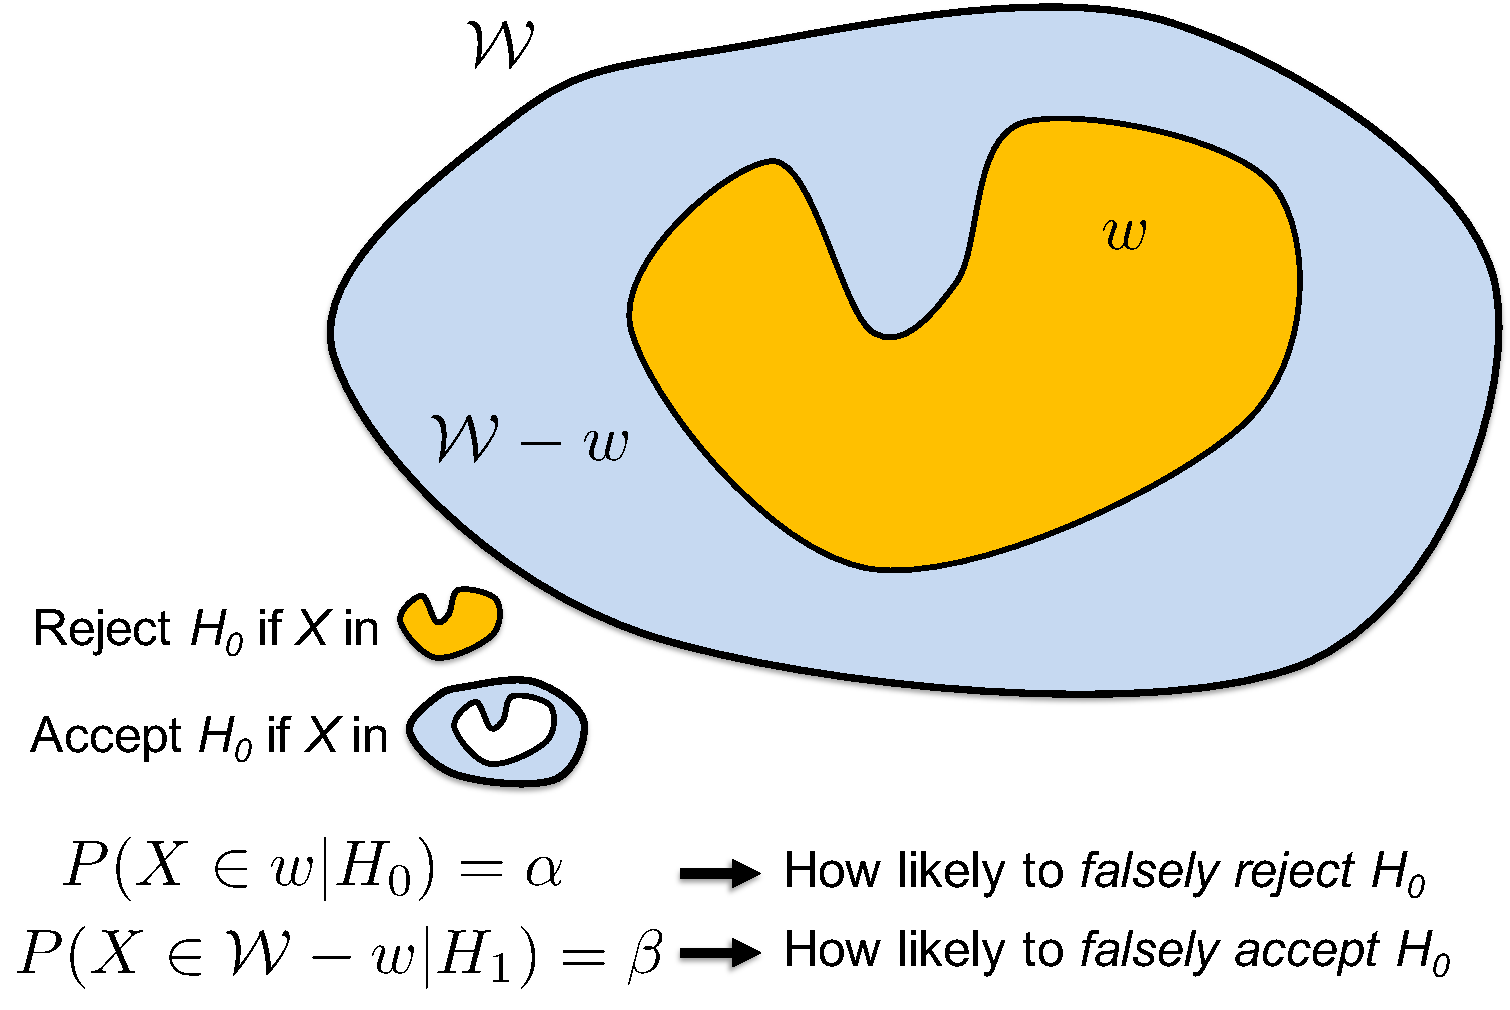
\includegraphics[width=0.6\textwidth]{figures/Hypotest/type12.pdf}
    \caption{Division of possibilities for the test statistic ($X$) into the yellow critical region $w$, and the blue region of acceptance $(\mathcal{W}-w)$. The probabilities that $X$ falls into the critical region, under the null hypothesis and alternate hypothesis are $\alpha$ and $(1-\beta)$, respectively.}
    \label{fig:htestregions}
\end{figure}
Some caution should be taken here. Remember we are dealing with two distinct simple hypotheses that cannot both simultaneously be true. Hence accepting one hypothesis means we are forced to reject the other (and vice versa). Particle physicists however don't usually talk about accepting hypotheses but rather rejecting them or not. This is because we rarely ever have a single test to establish that something is true, but we are often happy to use a single test to reject it - it's actually nearly always the same way with science, we tend to disprove theories  rather than prove them outright.

\begin{tcolorbox}[colback=backblue]
\textbf{Example:} Let's suppose we have a simple experimental setup that counts the number of charged particles, say electrons from a beam passing through a spark chamber. Say we can tune the beam to fire a fixed number of electrons at the chamber, and record the number of sparks $k$. When we ordered the detector, the manufacturer said it was 90\% efficient. So we set out to test our null hypothesis corresponding to $\epsilon=70\%$ hypothesis. Our test statistic will be $k$, and our critical region will correspond to values of $k\leq K$, where $K$ is the number satisfying, 
\begin{equation}
    \sum_{k=0}^{k=K} b(k;\epsilon,N),
\end{equation}
where $b(k;p,N)$ the our binomial probability distribution with success probability $\epsilon$ and $N$ trials. 

Suppose we run our experiment with 5000 electrons and observe 3420 sparks. Given this observation, we can think of Eqn.~\ref{eqn:testsize} as calculating the value of $\alpha$ where $K$ is our observation -- i.e instead of choosing $K$ such that $\alpha=0.05$, we  $K=83$ and compare the resulting value of $\alpha$ with 0.05. This is what is known as calculating a $p$-value (or tail probability) for a particular observation. We can calculate this numerically using a MC method - remember that convergence in probability requires a lot of MC. 

\begin{lstlisting}[style = Python]
import numpy as np
# parameters of the binomial probability distribution
N, eps=5000,0.70
# our observed number of sparks
K=3420

# generate MC pseudo observations
nMC=10000
random_k = np.random.binomial(N,eps,nMC)

# count the fraction of times we see a value of k
# less than or equal to K
pval = float(len([x for x in random_k if x<=K]))/nMC
print(pval)
\end{lstlisting}
We get a $p$-value of 0.0083.  This is smaller than 0.05 so based on this test we reject $H_0$. Of course we could have just calculated this $p$-value analytically but for more complicated test statistics, we will need to use MC methods.  
\end{tcolorbox}

In the example, we made our decision based on the $p$-value being smaller than 0.05, and we can check how often we would reject $H_0$, if it is true, based on this decision process. How often would we see a $p$-value smaller than 0.05? We can use MC to calculate it, but this time, we will use \textsf{binom} from the \textsf{scipy.stats} package (much faster). 
\clearpage
\begin{lstlisting}[style = Python]
import numpy as np
import matplotlib.pyplot as plt
# scipy has a lot of common pdfs for us to use
from scipy.stats import binom

# parameters of the binomial probability distribution
N, eps=5000,0.70

def calc_pval():
  # for a random observation K, we calculate the p-val
  # this time, just use in the handy scipy cdf
  K = np.random.binomial(N,eps)
  pval = binom.cdf(K,N,eps)
  return pval

nTests=10000
pvals = [calc_pval() for test in range(nTests)]
y,binEdges = np.histogram(pvals,bins=10)
bincenters = 0.5*(binEdges[1:]+binEdges[:-1])
menStd     = np.sqrt(y)
plt.bar(bincenters, y, width=0.025, yerr=menStd)
plt.xlabel("$p$-value")
plt.ylabel("Number of trials per bin")
plt.show()
\end{lstlisting}
This produces the plot shown in Figure~\ref{fig:p0dist}. You can see its flat. Actually this is not surprising since the distribution of the $p$-value under the null hypothesis is always flat\footnote{For a discrete test statistic its approximately flat but if our test statistic were continuous it really would be flat}! Immediately we can see then that by choosing to reject $H_0$ when the $p$-value is  exactly the probability that we would falsely reject $H_0$!

\begin{figure}
    \centering
    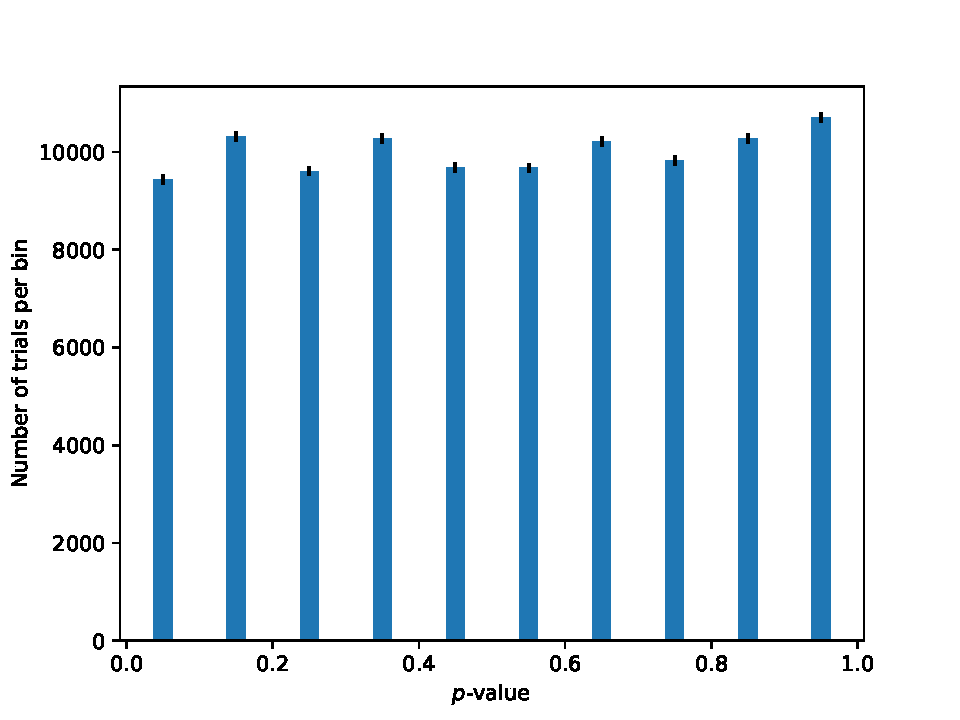
\includegraphics[width=0.8\textwidth]{figures/Hypotest/p0dist.pdf}
    \caption{Distribution of $p$-values under the hypothesis that $\epsilon=0.9$. The error bars indicate the standard deviation of the a Poisson whose mean equals the number of observed entries in each bin.}
    \label{fig:p0dist}
\end{figure}

Of course we might also be interested in finding a better estimate of the efficiency, rather than testing a single efficiency. All possible values of efficiencies $\epsilon \in [0,1]$ would then form a composite hypothesis. We'll come on to this later on, but first we need to introduce a fundamental concept in hypothesis testing - the likelihood function. 

\subsection{Likelihoods}
The likelihood function is a very powerful tool in statistics, and as a particle physicist will be your go-to when performing statistical inference. We've come across it already in Bayes' theorem when applied to experimental data (Eqn.~\ref{eqn:bayesexp}). 

The likelihood function $L$ is defined by, 
\begin{equation}\label{eqn:likelihood}
L(\theta) \propto P(X|\theta).
\end{equation}
The likelihood is defined for a fixed observation $X$ and is proportional to the probability to observe $X$, given a value of some parameter set $\theta$. The likelihood function is a \emph{function of the parameters} $\theta$. Note that we write a proportionality rather than an equality because the likelihood function is \emph{not} a probability density. In practice, we often only care about ratios of likelihoods for different values of the parameter(s) and hence we almost never care about this constant of proportionality. 

For $N$ independent observations $\mathbf{X}=\{X_{1},X_{2},...,X_{N}\}$, the likelihood function is, 
\begin{equation}\label{eqn:likelihoodprod}
L(\theta) := \prod_{i=1}^{N}f_{i}(X_{i};\theta),
\end{equation}
where $f_{i}$ are the p.d.f for each observation.

In HEP, we often make the distinction between  \emph{binned} likelihood and \emph{un-binned} likelihoods. To get the most out of the data, the un-binned likelihood is always better, however there may be restrictions that mean the binned likelihood is more appropriate. For example, if using MC simulation to estimate the distribution of some process, you may only be able to bin the simulation and hence you'll need to use a binned likelihood. Also, you might find that for computation, the binned likelihood is faster - this is usually the case if you have many events in your dataset. We'll see examples of both binned and un-binned likelihoods later, but for now, we need to cover an extremely important result, which unites likelihood functions and hypothesis testing.

\subsection{Neyman-Pearson Lemma}
Let's go back to the problem of finding the most powerful test of our null hypothesis $H_0$ against an alternate hypothesis $H_1$. As we've seen, we can state this problem as finding the \emph{best critical region} $w$. Let $\mathbf{X}$ be our observation (experimental data) and suppose it has a p.d.f $f(\mathbf{X};\theta)$, where $\theta=0$ represents the null hypothesis $H_0$ and $\theta=1$ represents the alternate hypothesis $H_1$. Note that I will reserve the notation $f(X|H)$ for only when $H$ represents a hypothesis for which $f(X|H)$ yields the distribution under which $X$ is distributed assuming $H$ is true -- very often in HEP, this is the same as setting some parameter values so that $f(X|H(\theta))=f(X;\theta)$ but i'll try not to confuse these notations. 

For a specific $\alpha$ we choose $w$ such that,
\begin{equation}\label{eqn:nptestsize}
    \int_{w}f(\mathbf{X};\theta_0)d\mathbf{X} = \alpha,
\end{equation}
and we want to find the region $w$ which maximises $1-\beta$. We can write Eqn.~\ref{eqn:power} as, 
\begin{eqnarray}\label{eqn:nppower}
    1-\beta & = &\int_{w}f(\mathbf{X};\theta_1)d\mathbf{X}\\
            & = &\int_{w}\frac{f(\mathbf{X};\theta_1)}{f(\mathbf{X};\theta_0)}f(\mathbf{X};\theta_0)d\mathbf{X}\\ 
            & = & E\left[\frac{f(\mathbf{X};\theta_1)}{f(\mathbf{X};\theta_0)}\bigg|\theta=\theta_0\right]_{w},
\end{eqnarray}
where the last line denotes the expectation value inside $w$, under the null hypothesis of the quantity,
\begin{equation}
\Lambda=\dfrac{f(\mathbf{X};\theta_1)}{f(\mathbf{X};\theta_0)}=\dfrac{L(\theta_1)}{L(\theta_0)}.
\end{equation}
This quantity is the ratio of the likelihood function, evaluated under the two hypotheses. The expectation in Eqn.~\ref{eqn:nppower} will be maximal when $w$ is chosen to contain the largest values of $\Lambda$. Thus, the best critical region is the set of points for which $\Lambda \geq c_{\alpha}\in \mathbb{R}$, where $c_{\alpha}$ satisfies Eqn.~\ref{eqn:nptestsize}. If $\Lambda>c_{\alpha}$, we would choose $H_{1}$, while $\Lambda \leq c_{\alpha}$ leads us to choose $H_0$. 

Often, given that this test is the most powerful, you will find that in HEP we use $\Lambda$ as \emph{the} test statistic, even if the hypotheses that we're testing are not simple ones. You should note however that the Neyman-Pearson lemma only applies to simple hypotheses and that $\Lambda$ is not necessarily the most optimal test statistic for other hypotheses -- in practice it turns out to have extensions which are extremely convenient so we still use ratios of likelihood functions ubiquitously in HEP. 


\subsection{Nuisance parameters}
So far we've talked about testing \emph{simple} hypotheses. As with most things in real life, the hypotheses that we want to test in particle physics are anything but simple. More often than not, we test \emph{composite} hypotheses against one another. Composite hypotheses can be thought of as a set of hypotheses that are parameterised by one (or more) parameters, often related to parameters of a physical model we are interested in. These parameters might correspond to the cross-section of some particle interaction process or the mass of a particle, or even some SUSY parameter like $\tan\beta$. In experimental particle physics, we also encounter parameters related to our experimental setup. These might be calibration coefficeints of the calorimeter, efficiencies on our event selection or the flux of a neutrino beam. Usually we are not so interested in defining the hypothesis with regards to all of these later parameters. We split the parameters of the model into two sets, $\theta=(\mu,\eta)$. The parameters $\mu$ are the \emph{parameters of interest} and typically correspond to the parameters that represent the set of hypotheses we are interested in testing. Instead, the parameters $\eta$ represent those parameters which we don't care about -- these are the \emph{nuisance parameters}. Typically, nuisance parameters are \emph{measured}, and we can think of those measured values as being random variables in their own right. The probability density function for them has two interpretations. Either you think of them as part of the likelihood itself, in which case particle physicists usually refer to them as \emph{external constraint terms}, or they simply represent our prior knowledge of the nuisance parameters -- practically this interpretation doesn't really matter but it can help when discussing with other particle physicists. Sometimes however, we have no prior knowledge about (one or more of) the nuisance parameters and in this case, they will not appear or will have flat priors.

Our composite hypotheses will be labelled as $H(\mu)=H\left(\mu,\eta(\mu)\right)$ meaning in order to specify the hypotheses corresponding to different values of $\mu$, we must make a choice of what to do with $\eta$, which can depend on the value of $\mu$. For dealing with experimental data, we will be using the likelihood function
and the choice boils down to one of two procedures, \emph{profiling} and \emph{marginalisation}. Typically, you will encounter profiling in frequentist procedures, and marginalisation in Bayesian procedures. There are however some procedures which have been used in the past that mix the two methods together (and it can make sense to do so), so we will just stick to calling them profiling or marginalising.

\paragraph{Profiled likelihoods}
Profiling the likelihood can sometimes be thought of selecting the ``best'' value of the nuisance parameters for any value of the parameters of interest. The definition of ``best'' here means that which maximises the likelihood for a particular value(s) of $\mu$. We'll see later that this choice will have useful implications, but for now, know that this is \emph{the choice} for frequentists. We start by taking twice the negative of the log-likelihood function,
\begin{equation}
    q(\mu,\eta)= -2\ln L(\mu,\eta).
\end{equation}
We then choose $\eta(\mu)$ as $\hat{\eta}_{\mu}$, which represents the values of $\eta$ for which $q$  minimized when evaluated at $\mu$. Specifically,
\begin{equation}
\hat{\eta}_{\mu} = \mathrm{arg min}_{\eta}\left\{q(\mu,\eta)\biggr|_{\mu}\right\},
\end{equation}
meaning we first fix $\mu$ and then find the values of $\eta$ which minimize $q$. If it's not clear, don't worry, we'll make it clear with an example soon. We then write the \emph{profiled log-likelihood} as,
\begin{equation}
q(\mu) = q(\mu,\hat{\eta}_{\mu}),
\end{equation}
to remove the $\eta$ dependence from the likelihood. Note that we've not specified the likelihood here, and we could have separated it into two components; $L(\mathrm{data}|\mu,\eta)\cdot L(\eta_{\mathrm{measured}}|\eta)$. The term $L(\eta_{\mathrm{measured}}|\eta)$ is the constraint term, which typically arises from some previous measurement of $\eta$, $\eta_{\mathrm{measured}}$. Often in HEP, we parameterize the likelihood so that $\eta_{\mathrm{measured}}=0$ and $L(\eta_{\mathrm{measured}}|\eta)\propto \prod_{i=1}^{M}\phi(0,1)$ for $M$ independent measurements (relying on the CLT to justify the choice of normal distributions), but this is just technicalities and we shouldn't get bogged down in this.

\paragraph{Marginalised posteriors}\label{sec:marginalised}
Marginalisation is the second way to deal with nuisance parameters. As before, we begin with the likelihood function $L(\mu,\eta)$. This time however, we separate out our prior knowledge of the nuisance parameters from the experimental data, plug into Bayes' theorem to obtain the posterior function and \emph{integrate} over the nuisance parameters,
\begin{equation}\label{eqn:bayesmargin}
P(\mu) = \frac{\int L(\mathrm{data}|\mu,\eta)\pi(\mu)\pi(\eta) d\eta}{P(\mathrm{data})},
\end{equation}
where $P(\mathrm{data})$ is the usual normalisation term $P(\mathrm{data})=\int\int L(\mathrm{data}|\mu,\eta)\pi(\mu)\pi(\eta) d\eta d\mu  $, and $\pi(\mu)$ and $\pi(\eta)$ are the \emph{prior probability densities} for $\mu$ and $\eta$.  Rather than choosing a single value of $\eta$ for each $\mu$, we've integrated over them, weighted according to the prior distribution. Thus the marginalised posterior is the expectation value of the posterior at each value of $\mu$. Here is where we need to be careful about the choice of priors, as our results can change depending on this choice. Any inference based on marginalised posteriors needs to include a study of the dependance on these priors. Typically in HEP, we tend to use \emph{flat} priors for $\mu$ and (similarly to the profiling case), normal priors for $\eta$. The latter is justified if there are external measurements of $\eta$, but ``flat'' for a parameter $\mu$ is not flat for a parameter $\mu^{2}$ -- it's not always obvious which is the more fundamental thing which we should have no prior knowledge about. For example, a cross-section is often proportional to a $\mathrm{(coupling)}^{2}$ but which one should be flat? The main thing is to make sure the final results are not very sensitive to this, otherwise explaining the choice of priors is vital for any paper.

In both cases we can now make statements about $H(\mu)$ either through the profiled likelihood $q(\mu)$ or the posterior $P(\mu)$ as the nuisance parameters $\eta$ have been eliminated. In the next section, we'll take a look at a concrete example to (hopefully) make it a more clear as to what we would do (practically) in both cases.

\subsection{A counting experiment}
To demonstrate profiling and marginalisation, we will use a very simple counting experiment. Counting experiments in HEP, simply mean that the observation (data) is just a single number $n$ -- the observed event count, and all of the model parameters are included inside the Poisson parameter $\lambda$. For a typical particle physics experiment, we want to study the rate of some particle X, produced in proton-proton collisions $pp\rightarrow\mathrm{X}$. We often have a theoretical prediction for the cross-section $\sigma(pp\rightarrow \mathrm{X})$, acceptance $A$ for our detector, efficiencies $\epsilon$ for our selection and a total integrated luminosity $l$. We usually introduce a scaling parameter $\mu$ that will parameterise different hypotheses. $\mu=1$ corresponds to the rate of the process being exactly as our theory colleagues predicted, while a value of $\mu=0$ means the process never occurs. There is almost always some background contribution $B$ so that the total rate can be written as,
\begin{equation}\label{eqn:lambdanom}
    \lambda(\mu) = \mu\sigma(pp\rightarrow \mathrm{X}) A\epsilon l + B,
\end{equation}
Nuisance parameters arise in counting experiments due to any one of the terms in Eqn.~\ref{eqn:lambdanom} being imprecisely known (or not at all). They are usually always parameterised using a \emph{log-normal} distribution. This is very common in HEP. If a random variable $\eta$ is distributed (or constrained by) a normal distribution with a mean of 0 and variance of 1, then $l=l_{0}(1+k)^{\eta}$ will be distributed as a log-normal and $\ln(l)$ will be normally distributed with a mean of $l_{0}$ and a variance of $k^{2}$. The nice thing about log-normals is that $l(\eta)$ parameterised in this way can \emph{never} be negative and hence neither can the Poisson mean. It's quite intuitive to think of this uncertainty having a relative effect - for example a 100\% uncertainty on $l$ means we know $l$ within a factor of 2 (we don't say that we think $l$ could be zero!). Furthermore, the smaller the value of $k$, the more $l(k)$ can be approximated by a normal distribution. Say then that our luminosity has some relative uncertainty $k$, we then write our Poisson mean as,
\begin{equation}
    \lambda(\mu,\eta) = \mu\sigma(pp\rightarrow \mathrm{X}) A\epsilon l(1+k)^{\eta} + B,
\end{equation}
Now we can use our two approaches to deal with this nuisance parameter. First, we'll take the profiling approach. The likelihood that we'll profile is,
\begin{equation}\label{eqn:lhcounting}
    L(\mu,\eta) = \lambda(\mu,\eta)^{n}e^{-\lambda}\cdot e^{-\frac{1}{2}\eta^{2}},
\end{equation}
where we've dropped any terms that are constant in $\mu$ and $\eta$. The term  $e^{-\frac{1}{2}\eta^{2}}$ is our constraint term for $\eta$. We now take twice the negative log,
\begin{equation}
    q(\mu,\eta) = -2\ln L(\mu,\eta) = \eta^{2}+2\lambda(\mu,\eta)-2n\ln\lambda(\mu,\eta).
\end{equation}
Minimizing $q(\mu,\eta)$ is the same as maximising $L(\mu,\eta)$. We could use any number of minimisation programs to do this for us, but since this problem is quite simple, we can code up a simple Newton method to find the solution to $q'=\frac{\partial q}{\partial \eta}=0$. In the Newton algorithm, from an initial starting point, $\eta_0$, the next point is proposed as $\eta_1=\eta_0-\frac{q'(\eta_{0}}{q''(\eta_0)}$. We iterate until $|q'|<\delta$ picking some tolerance. We can analytically calculate,
\begin{eqnarray}
    q'  =  \frac{\partial q}{\partial \eta} & = &   
    2\eta 
    +2\frac{\partial\lambda}{\partial \eta} 
    - \frac{2n}{\lambda}\frac{\partial\lambda}{\partial \eta} = 
    2\eta 
    + 2\ln(1+k) \left(\lambda-B\right)
    -2n\ln(1+k)\frac{\lambda - B}{\lambda}\\
    q''  =  \frac{\partial ^{2}q}{\partial \eta^{2}} 
    & = &   
    2 
    + 2\ln(1+k)\frac{\partial\lambda}{\partial \eta} 
    - 2n\ln(1+k)\left( \frac{B}{\lambda^{2}}\frac{\partial\lambda}{\partial \eta}  \right)
    = 
    2 
    + 2(\ln(1+k))^{2}\left(\lambda-B\right)\left( 1-\frac{nB}{\lambda^{2}}\right),
\end{eqnarray}

where we've used the fact that $\frac{\partial\lambda}{\partial \eta} =\ln(1+k)(\lambda-B)$.

For each value of $\mu$, we can find $\hat{\eta}_{\mu}$ as the solution to $\frac{\partial q}{\partial \eta}\biggr|_{\mu}=0$.

For marginalisation, we again start with the likelihood, but this time, we maintain all of the terms
\begin{eqnarray}
    L(n|\mu,\eta) & = & \frac{\lambda(\mu,\eta)^{n}}{n!}e^{-\lambda}\\
    P(\eta) & = & \frac{1}{\sqrt{2\pi}}e^{-\frac{1}{2}\eta^{2}}\\
    \pi(\mu) & = & \begin{cases}
                \frac{1}{15} & \mu \in (-1,15) \\
                0 & \mathrm{else,}
                \end{cases}
\end{eqnarray}
and we simply plug these into Eqn.~\ref{eqn:bayesmargin} to obtain the posterior $P(\mu)$. Here we've chosen a wide prior for $\mu$ so as to not affect the posterior.

Now suppose you've called your colleagues up in Durham and they've sent over a theoretical prediction for the cross-section $\sigma(pp\rightarrow \mathrm{X}) = 0.01$pb. You also know your apparatus well and know that for this process, the efficiency of your selection will be $\epsilon=0.9$ and the acceptance $A=0.5$. You collide protons until you reach a total integrated luminosity of $l=100\mathrm{pb}^{-1}$. You don't know the luminosity perfectly, but it has been measured to within 10\%, so $k=0.1$. The backround rate is known to be $B=0.5 $. After running the experiment, we observe 2 events. Below is some code which defines this setup. We can save this in a file called \textsf{model.py} so that we can import it later rather than redefine each time.
\begin{lstlisting}[style = Python]
sigma_TH = 0.01
A = 0.5 
eff = 0.9 
l = 100. 
k = 0.1 
B = 1.0
n   = 2

# Poisson mean
def lamb(mu,eta):
  return mu*eff*A*l*((1+k)**eta)*sigma_TH + B
\end{lstlisting}

To calculate the profile likelihood in our simple counting experiment, we use the Newton method. Figure~\ref{fig:profiledlikelihoodex_counting} can be produced 
by following the notebook \href{https://github.com/nucleosynthesis/PGStatistics/blob/main/notebooks/ProfilingVsMarginalisation.ipynb}{\textsf{ProfilingVsMarginalisation.ipynb}}.

\begin{figure}[hbt!]
    \centering
    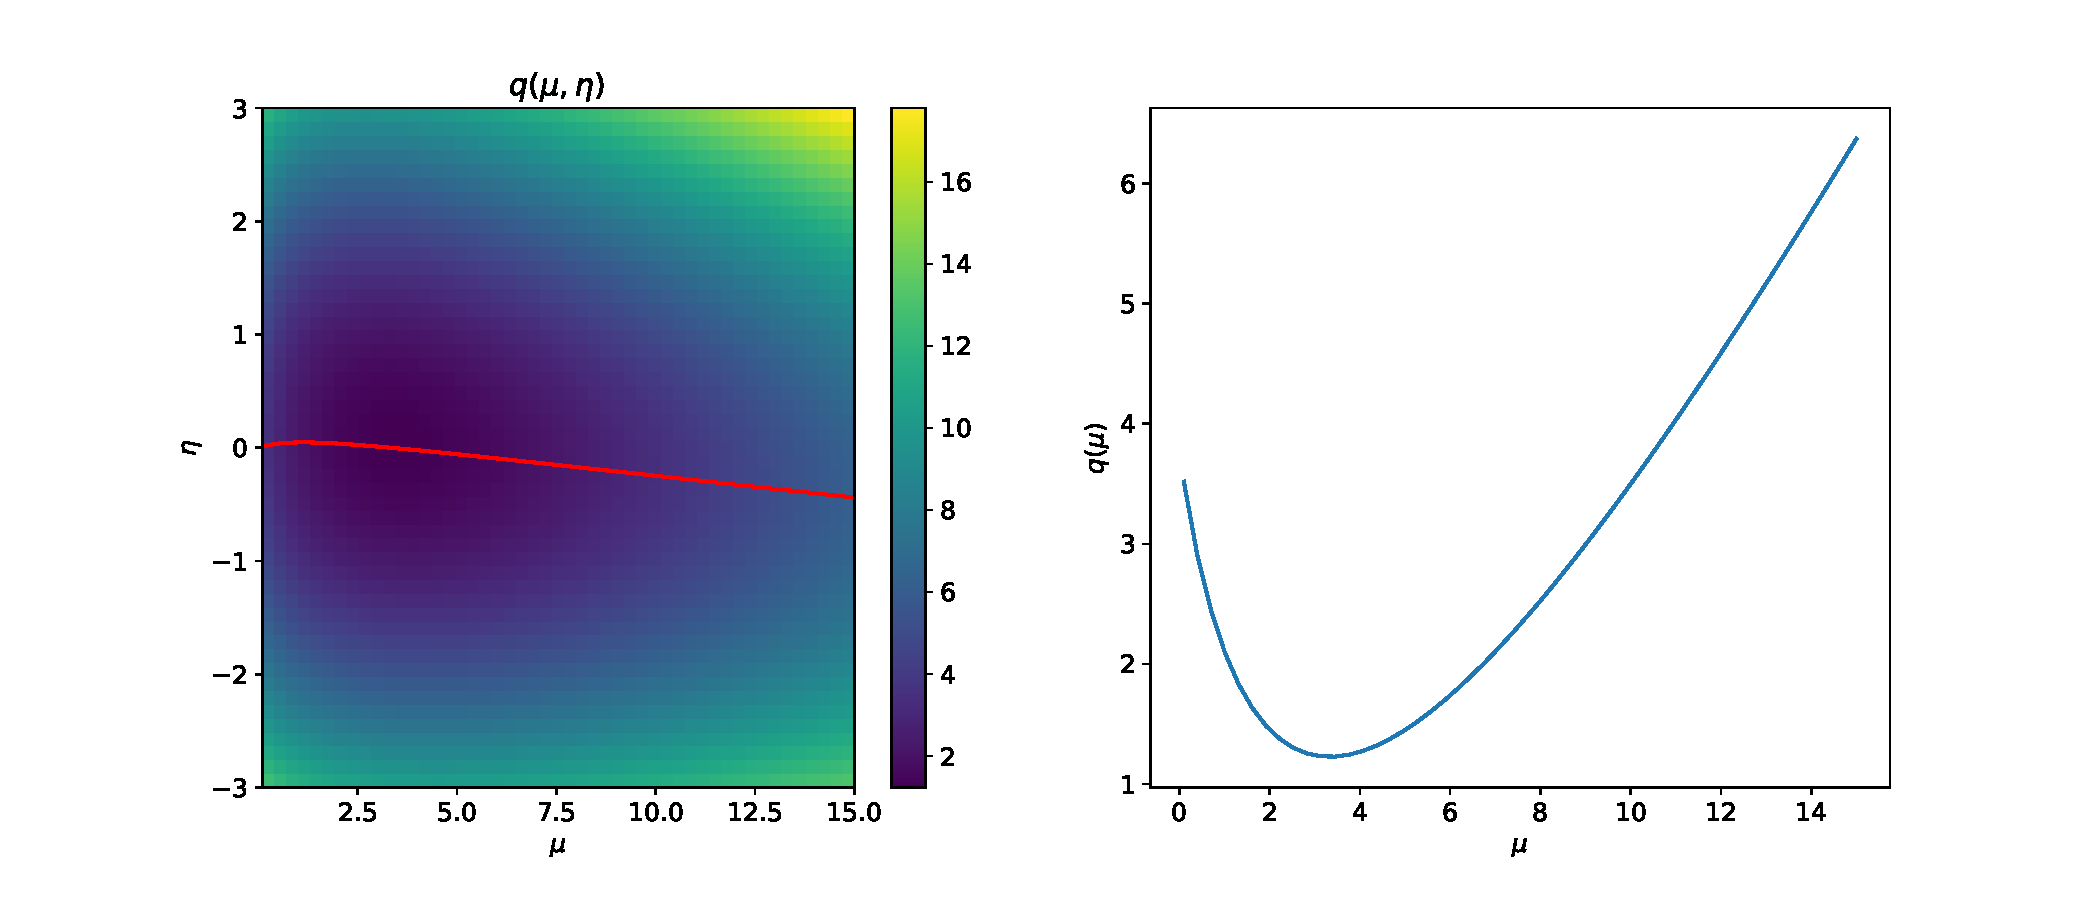
\includegraphics[width=\textwidth]{figures/Hypotest/prof_lh_ex.pdf}
    \caption{Left: Twice negative log-likelihood function for the counting experiment vs 
    $\mu$ and $\eta$. The red line shows the profiled value of the nuisance parameter at each value of $\mu$ $\hat{\eta}_{\mu}$. Right: the profiled log-likelihood function $q(\mu)$.}
    \label{fig:profiledlikelihoodex_counting}
\end{figure}

If instead, we want to obtain the marginalised posterior function, 
we can use the \textsf{scipy.integrate.quad} methods 
to perform the integration numerically. An example code for 
producing the marginalised posterior is below, and the output 
from the code is shown in Figure~\ref{fig:marginalised_ex_counting}. 
Again, you can follow the 
\href{https://github.com/nucleosynthesis/PGStatistics/blob/main/notebooks/ProfilingVsMarginalisation.ipynb}{\textsf{ProfilingVsMarginalisation.ipynb}} 
notebook to see how this works. In that notebook, the posterior distribution is also computed 
using the Markov chain MC method that we covered in section~\ref{sec:MarkovChain}. 


\begin{figure}[hbt!]
    \centering
    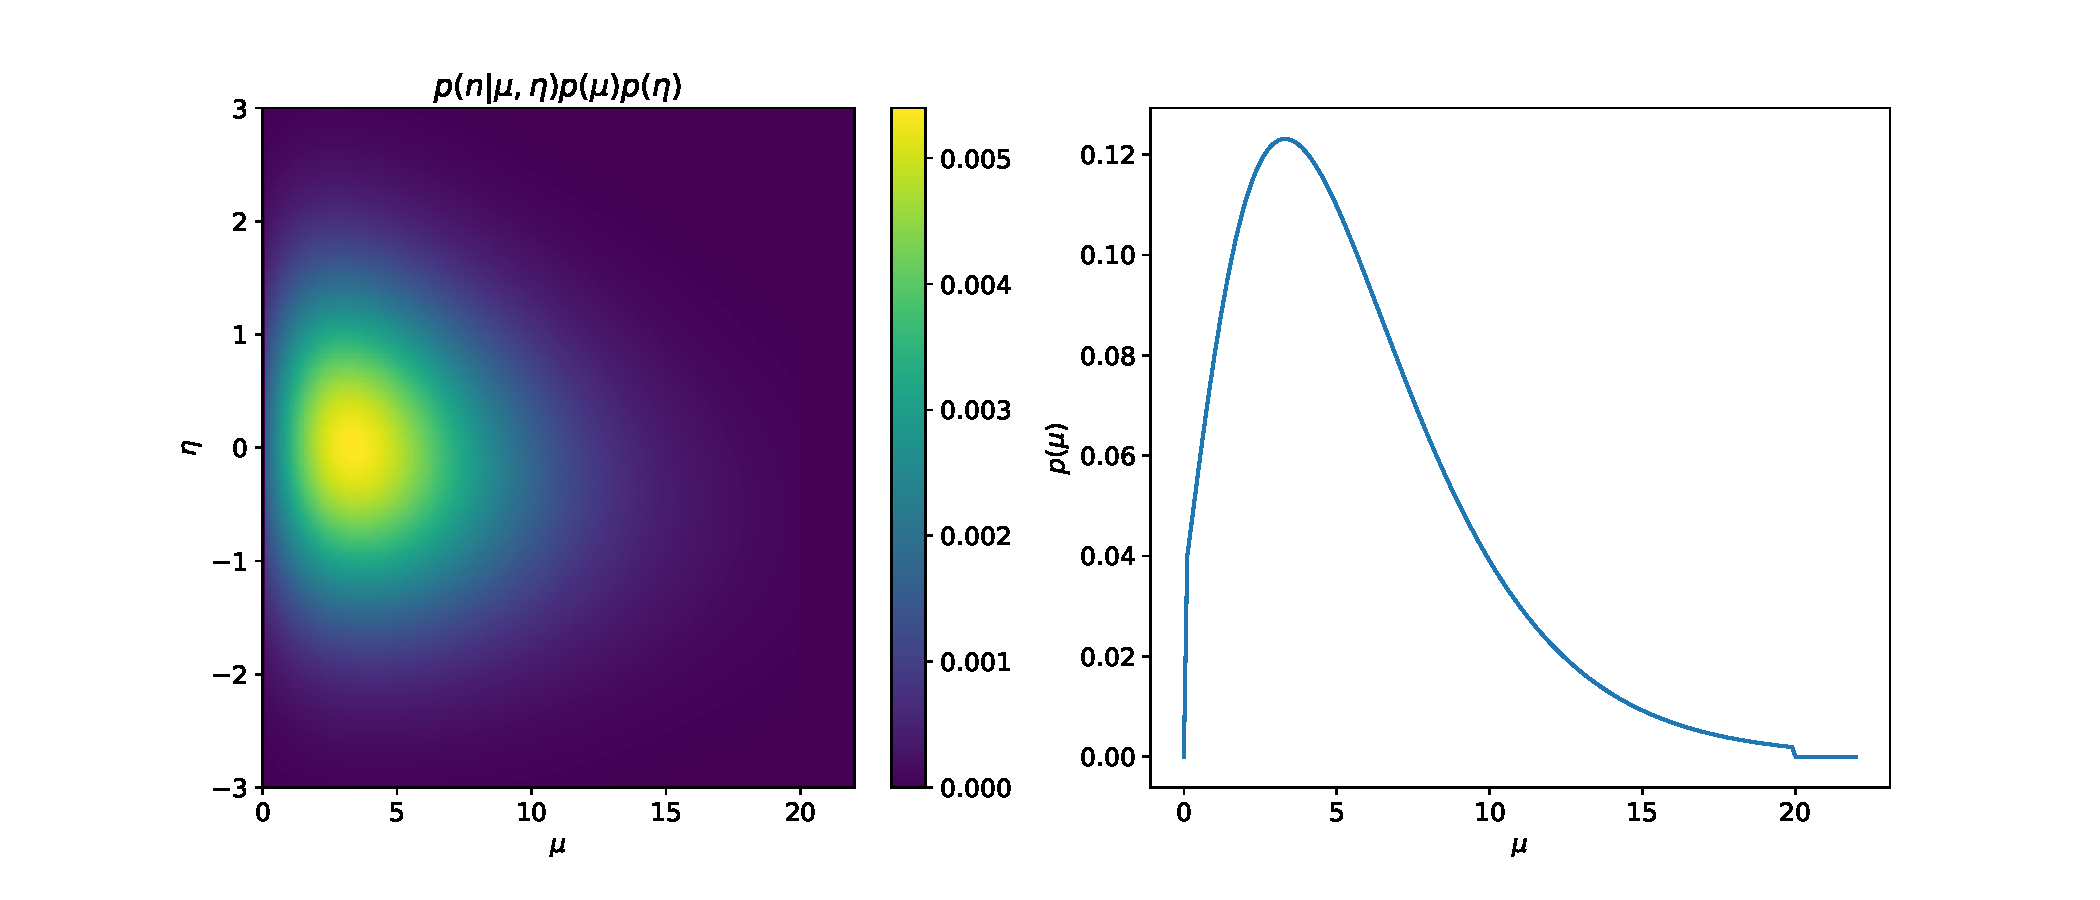
\includegraphics[width=\textwidth]{figures/Hypotest/marginalised_lh_ex.pdf}
    \caption{Left: Likelihood function multipltied by priors on $\mu$ and $\eta$ for the counting experiment vs $\mu$ and $\eta$.  Right: the marginalised posterior function $P(\mu)$.}
    \label{fig:marginalised_ex_counting}
\end{figure}

For Bayesians, having the posterior, now only as a function of the parameter of interest, is enough to perform statistical inference, such as hypothesis tests. One question that you'll probably have to ask (unfortunately) is which hypotheses can we exclude (reject) with some error rate $\alpha$ given the data observed? In the case where we have parameterised the set of hypotheses with parameter $\mu$, we can ask which values of $\mu$ can be rejected. For an example such as the counting experiment, we can also ask what the \emph{largest} value of $\mu$ (and hence which set of $H(\mu)$) can be rejected with error rate $\alpha$. This is referred to as an \emph{upper limit} on $\mu$, and the Bayesian would calculated it as $\mu_{\mathrm{up}}$ satisfying, 
\begin{equation}
    \int_{-\infty}^{\mu_{\mathrm{up}}}P(\mu)d\mu = 1-\alpha,
\end{equation}
where in practice, one rarely needs to use $-\infty$ as a lower bound. With this, we can reject all hypotheses $\left\{H(\mu):\mu>\mu_{\mathrm{up}}\right\}$ at an error rate of $\alpha$ or less. 

Bayesians would say that this is the upper limit on $\mu$ with $100\times(1-\alpha)$\% credibility. The equivalent from frequentists would be to determine the upper limit on $\mu$ with $100\times(1-\alpha)$\% confidence level. We'll come back to credible intervals and confidence intervals later on. But for now, we need to do a bit more work for the frequentists, and at the same time we'll introduce the standard tools for setting upper limits in HEP. 

\subsection{Upper limits and common HEP test statistic}
As we've mentioned already, profiled likelihoods (and ratios of them) are very common in hypothesis testing, due to the Neyman-Pearson lemma. In HEP, and in particular at the LHC, there is a standard test statistic used to set upper limits on cross-sections/signal-rates. The first step, is to identify a signal scaling parameter as we had done in the previous section -- $\mu$. Typically when searching for a new phenomena. 

We mentioned the idea of excluding a particular hypothesis $H(\mu)$ at a given confidence level $1-\alpha$ by finding an upper limit on $\mu$. We can think of this as a series of tests, one for each value of $\mu$
and deciding whether to reject it or not, with a given error rate $\alpha$. In each of these tests, our \emph{null} hypothesis is $H(\mu)$ since we are asking whether or not we can reject it. Clearly $H(0)$ is the \emph{background only} hypothesis, and usually we parameterise the signal such that $H(1)$ corresponds to some theoretical prediction. If we exclude all $\mu\geq 1$ (i.e $\mu_{\mathrm{up}}<1)$ , we have excluded this theoretical model. 

We also need an alternate hypothesis, and for that, we use the $\emph{best}$ value of $\mu$ given the observed data - $\hat{\mu}$. Again, this means finding the value of $\mu$ which (minimises) maximises the (log)likelihood function. The test statistic that we use is,
\begin{equation}
    t_{\mu} = \begin{cases}
                q(\mu,\hat{\eta}_{\mu})-q(\hat{0},\hat{\eta}_{0})    & \hat{\mu} < 0 \\
                q(\mu,\hat{\eta}_{\mu})-q(\hat{\mu},\hat{\eta})    & \hat{\mu} \in (0,\mu] \\
                0               & \hat{\mu}>\mu,
                \end{cases}
\end{equation}
where we've introduced $\hat{\eta}$ to mean the \emph{global} best nuisance parameter values for any value of $\mu$. The value $q(\hat{\mu},\hat{\eta})$ is the \emph{global} minimum of $q(\mu,\eta)$. Note that there are 3 cases. The second case, is exactly our profiled likelihood, offset by the global value. The first case, imposes a constraint that $\mu<0$ is \emph{unphysical} and the third case enforces an \emph{upper limit} on $\mu$. 

For each value of $\mu$, we calculate the $p$-value, 
\begin{equation}
    p_{\mu} = \int_{t^{\mathrm{obs}}_{\mu}}^{+\infty} f(t_{\mu}|H(\mu))dt_{\mu},
\end{equation}
where $f(t_{\mu}|H(\mu))$ is the distribution of $t_{\mu}$ under the hypothesis $H(\mu)$ is true typically calculated using MC methods, and $t^{\mathrm{obs}}_{\mu}$ are the values of $t_{\mu}$ for the observed data. This particular test statistic has the added bonus that the distribution can be determined analytically in the asymptotic (normal approximation) limit, meaning we don't need to use MC to determine $f(t_{\mu}|H(\mu))$\footnote{You can find these formula in the paper ``Asymptotic formulae for likelihood-based tests of new physics'', \href{https://arxiv.org/abs/1007.1727}{DOI: 10.1140/epjc/s10052-011-1554-0}}, saving us a lot of computing time.

Let's apply this to our simple example counting experiment using a MC method. The first thing is to decide how we are going to generate pseudo-experiments (toys) to determine $f(t_{\mu}|H(\mu))$. We have again encountered the problem that $H(\mu)$ is defined only for a fixed choice of the nuisance parameters $\eta$. Once again, we'll turn to our choice of the \emph{best} values, meaning we will pick those which minimises $q(\mu,\eta)$ for a given value of $\mu$ given our observed data. We already calculated these, it's the red line in Figure~\ref{fig:profiledlikelihoodex_counting} -$\hat{\eta}_{\mu}$. For each toy, we want to generate a random value of the observation $n'$, given $\mu,\hat{\eta}_{\mu}$ and a value of $\eta'$ which represents the random outcome for $\eta$ our luminosity measurement - remember, in the frequentist view, the value that we obtained can also be interpreted as a random variable with a known distribution $\eta{^{\prime}}\sim\phi(\hat{\eta}_{\mu},1)$ -- our observed data then becomes $(n^{\prime},\eta^{\prime})$. We need to modify the likelihood function of Eqn.~\ref{eqn:lhcounting} for each toy slightly to read, 
\begin{equation}
    L(\alpha,\eta) = L(n^{\prime},\eta^{\prime}) = \lambda(\mu,\eta)^{n\prime}e^{-\lambda}\cdot e^{-\frac{1}{2}(\eta-\eta^{\prime})^{2}},
\end{equation}
For each toy, we can then calculate $t_{\mu}$ using this data in the likelihood function and histogram the results. Note that for each toy, we will find different values of $\hat{\mu}$ and $\hat{\eta}_{\mu}$! 

Follow the \href{https://github.com/nucleosynthesis/PGStatistics/blob/main/notebooks/FrequentistUpperLimits.ipynb}{FrequentistUpperLimits.ipynb} notebook for an example where we calculate the 95\% confidence level upper limit for $\mu$ for our simple counting experiment. 

Figure~\ref{fig:tmu_example} shows example distributions of $t_{\mu}$ for the hypothesis $H(\mu=8)$ and $H(\mu=15)$. The red lines indicate the observed value $t_{\mu}^{\mathrm{obs}}$, which is used to calculate $p_{8}$ and $p_{15}$. Now, we need to calculate this distribution, and hence $p_{\mu}$ for a range of values of $\mu$. Once this is done, we can read of the value of $\mu_\mathrm{up}$ at a $100\times(1-\alpha)$ confidence level as the value of $\mu$ for which $p_{\mu}$ crosses $(1-\alpha)$. 

The result is shown in Figure~\ref{fig:pmu_example}. From here, we can find the 95\% CL upper limit by reading off where the black line crosses 0.05. 

\begin{figure}
    \centering
    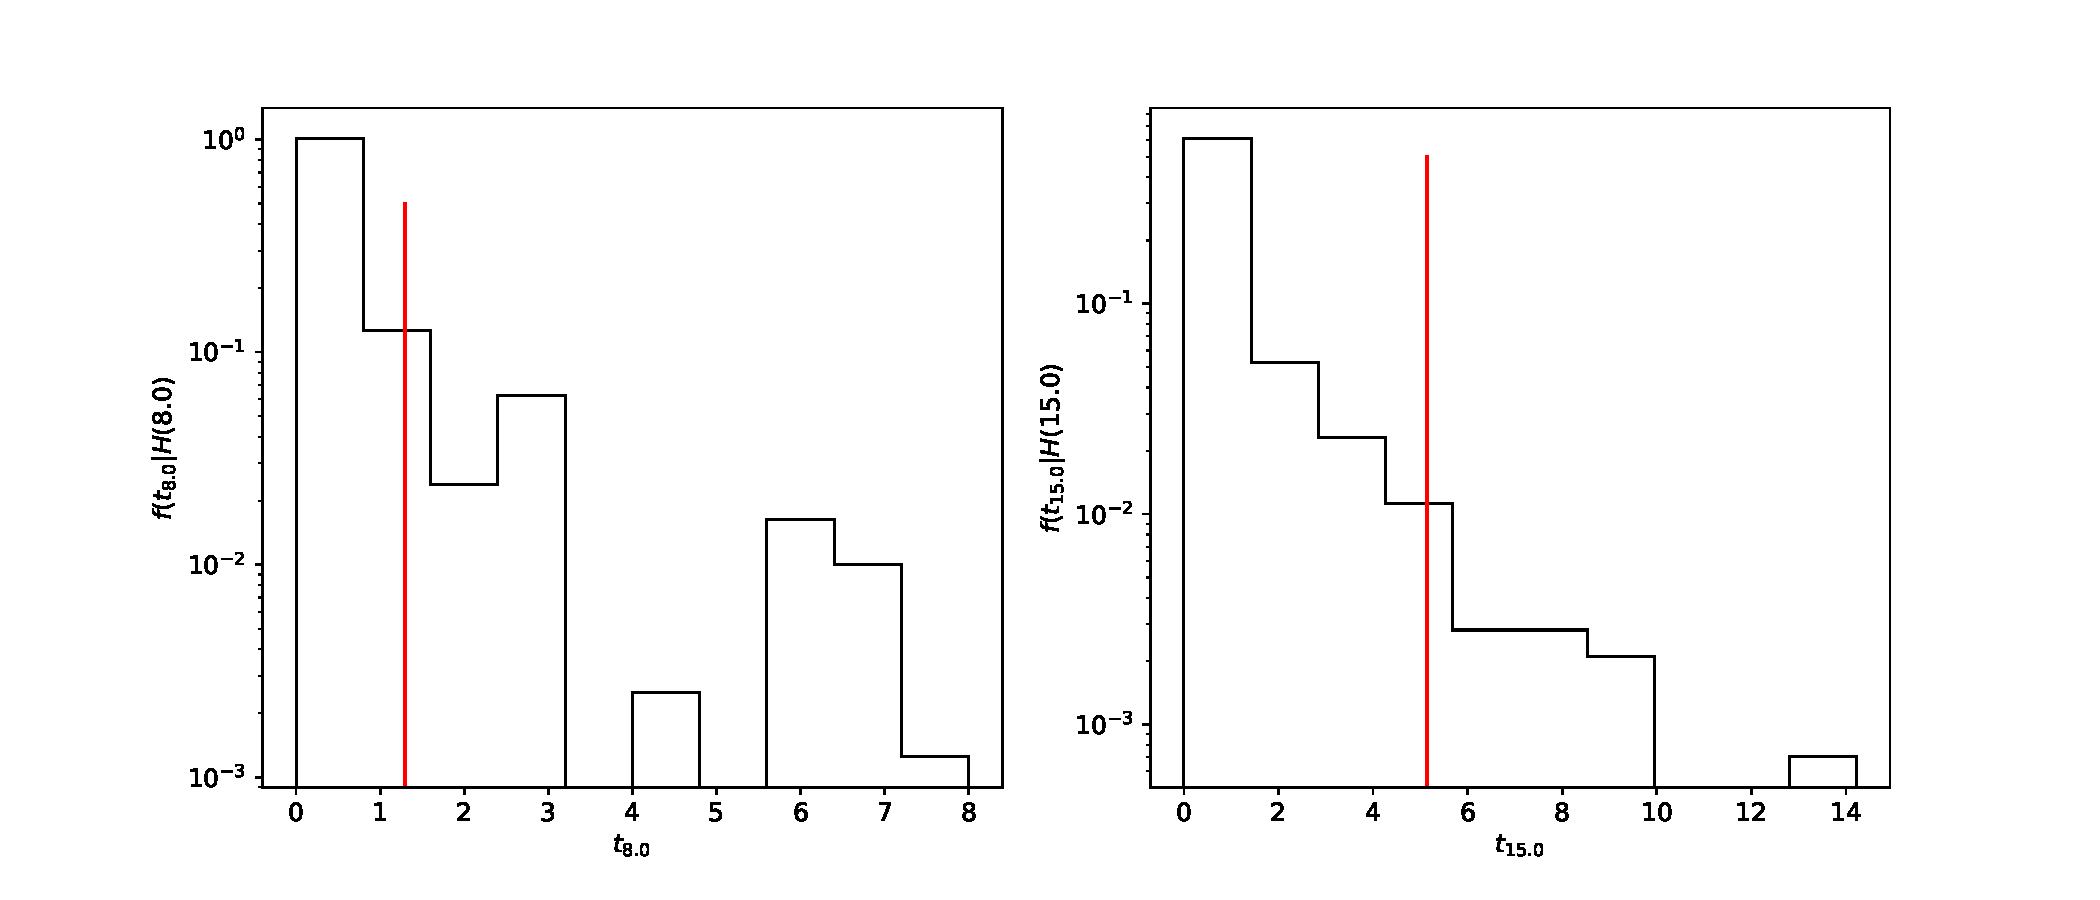
\includegraphics[width=\textwidth]{figures/Hypotest/p10.pdf}
    \caption{Example distribution of $t_{\mu}$ for $\mu=8$ (left) and $\mu=15$ (right) . The vertical red line indicates the value of  $t_{8}^{obs}$ and $t_{15}^{obs}$.}
    \label{fig:tmu_example}
\end{figure}

\begin{figure}
    \centering
    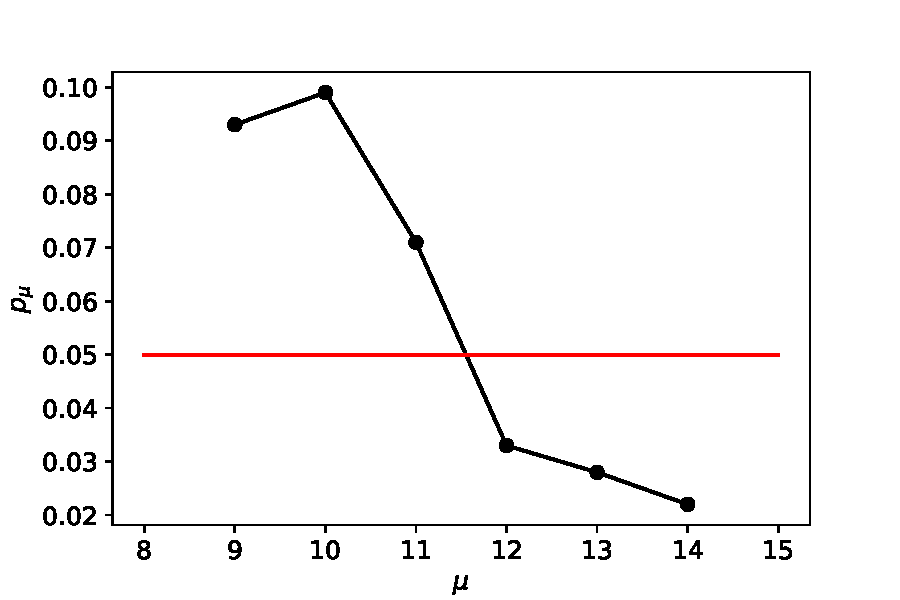
\includegraphics[width=\textwidth]{figures/Hypotest/scan_pmu.pdf}
    \caption{
    $p_{\mu}$ vs $\mu$. The horizontal red line lets us read off the value of $\mu_{\mathrm{up}}$ at the 95\% confidence level, given our observation.}
    \label{fig:pmu_example}
\end{figure}

In most real-life scenarios, you will deal with many nuisance parameters rather than just a few. In this case, I have used the \textsf{minimize} function from \textsf{scipy.optimize} (there are others like \textsf{MINUIT}, etc) which uses   gradient descent or even stochastic based routines to find the (log)likelihood extrema. For marginalisation, integration is typically performed using MC methods such as the Markov chain approach. As I mentioned at the start, these lectures aren't about these tools, but feel free to ask me/your colleagues about them when you start your Ph.D research. 

You will most likely come across the $CL_{S}$ criterion during your Ph.D. Using  the $CL_{S}$ criterion  means that instead of basing the test on $p_{\mu}$, we base it on the value of $CL_{S}=\frac{p_{\mu}}{1-p_{b}}$ compared to $\alpha$, where 
\begin{equation}
    p_{b} = \int_0^{t^{\mathrm{obs}}_{\mu}}  f(t_{\mu}|H(0))dt_{\mu}.
\end{equation}
We won't dwell on this too much but you should know that $CL_{S}$ is known to \emph{over-cover} (what does that even mean? Don't worry, we'll get to it) and is designed to avoid excluding a signal hypothesis when the data disagrees with the background-only hypothesis and the signal plus background hypothesis, when the two look very similar. Now that I've started to introduce words like \emph{cover}, we should move on to explaining credible/confidence intervals and the concept of $\emph{coverage}$. 